% answers.tex —— 2021 年·全国乙卷·理科 · 参考答案与详细解析片段
% 由 tools/generate_projects.py 依来源总账自 2021/2021_数学真题_全国乙理_试题.md + 2021/2021_数学真题_全国乙理_解析正文.md + 2021/2021_数学真题_全国乙理_答案要点.md 生成，勿手改（改源 MD 后重跑）


\begin{gktip}
全部答案与解析依据上游 PDF 题面独立重建，非官方答案或解析。
\end{gktip}

\gkpart{一、选择题}

\begin{answer}
\gksolhead{1}{}

\textbf{题目}：

设 $2(z+\bar z)+3(z-\bar z)=4+6\mathrm i$，则 $z=$\mbox{（　　）}

\begin{gkopts}(4)
\task A．$1-2\mathrm i$
\task B．$1+2\mathrm i$
\task C．$1+\mathrm i$
\task D．$1-\mathrm i$
\end{gkopts}

\Needspace{4\baselineskip}
\textbf{解析}

令 $z=x+\mathrm iy$，则 $z+\bar z=2x$、$z-\bar z=2\mathrm iy$。原式化为 $4x+6\mathrm iy=4+6\mathrm i$，所以 $x=y=1$，$z=1+\mathrm i$，选 C。

\gkanswer{答案：C}

\end{answer}
\begin{answer}
\gksolhead{2}{}

\textbf{题目}：

已知集合 $S=\{s\mid s=2n+1,\ n\in\mathbf Z\}$，$T=\{t\mid t=4n+1,\ n\in\mathbf Z\}$，则 $S\cap T=$\mbox{（　　）}

\begin{gkopts}(4)
\task A．$\varnothing$
\task B．$S$
\task C．$T$
\task D．$\mathbf Z$
\end{gkopts}

\Needspace{4\baselineskip}
\textbf{解析}

$S$ 是所有奇整数，$T$ 是所有模 $4$ 余 $1$ 的整数。每个 $4n+1$ 都可写成 $2(2n)+1$，所以 $T\subset S$，交集是 $T$，选 C。

\gkanswer{答案：C}

\end{answer}
\begin{answer}
\gksolhead{3}{}

\textbf{题目}：

已知命题 $p:\exists x\in\mathbf R,\ \sin x<1$；命题 $q:\forall x\in\mathbf R,\ \mathrm e^{|x|}\geqslant1$，则下列命题中为真命题的是\mbox{（　　）}

\begin{gkopts}(4)
\task A．$p\land q$
\task B．$\neg p\land q$
\task C．$p\land\neg q$
\task D．$\neg(p\lor q)$
\end{gkopts}

\Needspace{4\baselineskip}
\textbf{解析}

$x=0$ 时 $\sin x=0<1$，故存在命题 $p$ 为真。对任意实数 $x$，$|x|\geqslant0$，于是 $\mathrm e^{|x|}\geqslant1$，全称命题 $q$ 也为真。真命题为 $p\land q$，选 A。

\gkanswer{答案：A}

\end{answer}
\begin{answer}
\gksolhead{4}{}

\textbf{题目}：

设函数 $f(x)=\dfrac{1-x}{1+x}$，则下列函数中是奇函数的是\mbox{（　　）}

\begin{gkopts}(4)
\task A．$f(x-1)-1$
\task B．$f(x-1)+1$
\task C．$f(x+1)-1$
\task D．$f(x+1)+1$
\end{gkopts}

\Needspace{4\baselineskip}
\textbf{解析}

逐项化简，$f(x-1)+1=\dfrac{2-x}{x}+1=\dfrac2x$，其定义域为 $\mathbf R\setminus\{0\}$，且 $\dfrac2{-x}=-\dfrac2x$，因此它是奇函数，选 B。

\gkanswer{答案：B}

\end{answer}
\begin{answer}
\gksolhead{5}{}

\textbf{题目}：

在正方体 $ABCD-A_1B_1C_1D_1$ 中，$P$ 为 $B_1D_1$ 的中点，则直线 $PB$ 与 $AD_1$ 所成角为\mbox{（　　）}

\begin{gkopts}(4)
\task A．$\dfrac{\pi}{2}$
\task B．$\dfrac{\pi}{3}$
\task C．$\dfrac{\pi}{4}$
\task D．$\dfrac{\pi}{6}$
\end{gkopts}

\Needspace{4\baselineskip}
\textbf{解析}

设正方体棱长为 $1$，取
$A=(0,0,0),B=(1,0,0),D=(0,1,0),A_1=(0,0,1)$。
则 $B_1=(1,0,1),D_1=(0,1,1)$，$P=(1/2,1/2,1)$。方向向量可取
$\overrightarrow{PB}=(1/2,-1/2,-1)$ 与 $\overrightarrow{AD_1}=(0,1,1)$。

点积为 $-3/2$，两向量模长之积为 $\sqrt3$，故两直线所成角 $\theta$ 满足 $\cos\theta=|{-3/2}|/\sqrt3=\sqrt3/2$，即 $\theta=\pi/6$，选 D。

\gkanswer{答案：D}

\end{answer}
\begin{answer}
\gksolhead{6}{}

\textbf{题目}：

将 $5$ 名北京冬奥会志愿者分配到花样滑冰、短道速滑、冰球和冰壶 $4$ 个项目进行培训，每名志愿者只分配到 $1$ 个项目，每个项目至少分配 $1$ 名志愿者，则不同的分配方案共有\mbox{（　　）}

\begin{gkopts}(4)
\task A．$60$ 种
\task B．$120$ 种
\task C．$240$ 种
\task D．$480$ 种
\end{gkopts}

\Needspace{4\baselineskip}
\textbf{解析}

四个指定项目都要有人，五人中恰有一个项目分到两人。先选这个项目有 $4$ 种，再从五人中选两人有 $\binom52$ 种，其余三人分配到其余三项目有 $3!$ 种。总数
$4\binom52 3!=240$，选 C。

\gkanswer{答案：C}

\end{answer}
\begin{answer}
\gksolhead{7}{}

\textbf{题目}：

把函数 $y=f(x)$ 图象上所有点的横坐标缩短到原来的 $\dfrac12$ 倍，纵坐标不变，再把所得曲线向右平移 $\dfrac{\pi}{3}$ 个单位长度，得到函数 $y=\sin\left(x-\dfrac{\pi}{4}\right)$ 的图象，则 $f(x)=$\mbox{（　　）}

\begin{gkopts}(1)
\task A．$\sin\left(\dfrac{x}{2}-\dfrac{7\pi}{12}\right)$
\task B．$\sin\left(\dfrac{x}{2}+\dfrac{\pi}{12}\right)$
\task C．$\sin\left(2x-\dfrac{7\pi}{12}\right)$
\task D．$\sin\left(2x+\dfrac{\pi}{12}\right)$
\end{gkopts}

\Needspace{4\baselineskip}
\textbf{解析}

横坐标缩短到原来的 $1/2$，对应函数变为 $f(2x)$；再向右平移 $\pi/3$ 后为 $f(2x-2\pi/3)$。因此
$f(2x-2\pi/3)=\sin(x-\pi/4)$。
令 $u=2x-2\pi/3$，则 $x=u/2+\pi/3$，所以
$f(u)=\sin(u/2+\pi/12)$，选 B。

\gkanswer{答案：B}

\end{answer}
\begin{answer}
\gksolhead{8}{}

\textbf{题目}：

在区间 $(0,1)$ 和 $(1,2)$ 中各随机取 $1$ 个数，则两数之和大于 $\dfrac74$ 的概率为\mbox{（　　）}

\begin{gkopts}(4)
\task A．$\dfrac79$
\task B．$\dfrac{23}{32}$
\task C．$\dfrac9{32}$
\task D．$\dfrac29$
\end{gkopts}

\Needspace{4\baselineskip}
\textbf{解析}

令两次抽取的数分别为 $x\in(0,1)$、$y\in(1,2)$。概率等于单位正方形中区域 $y>7/4-x$ 的面积。对 $0<x<3/4$，有利的 $y$ 长度为 $x+1/4$；对 $3/4<x<1$，全部 $y$ 都有利。因此
$P=\int_0^{3/4}(x+\tfrac14)\,dx+\int_{3/4}^1 1\,dx=\tfrac{23}{32}$，选 B。

\gkanswer{答案：B}

\end{answer}
\begin{answer}
\gksolhead{9}{}

\textbf{题目}：

魏晋时期刘徽编写的《海岛算经》是关于测量的数学著作，其中第一题是测量海岛的高。如图，点 $E,H,G$ 在水平线 $AC$ 上，$DE$ 和 $FG$ 是两个垂直于水平面且等高的测量标杆的高度，称为“表高”，$EG$ 称为“表距”，$GC$ 和 $EH$ 都称为“表目距”，$GC$ 与 $EH$ 的差称为“表目距的差”，则海岛的高 $AB=$\mbox{（　　）}
\nopagebreak[4]
\begin{center}% 2021 全国乙卷理科第 9 题：海岛测高示意图；逻辑图名 2021-national-b-science-t09-island
% 依据 PDF 第 1 页；A、E、H、G、C 共线，DE=FG，B-D-H 与 B-F-C 共线。
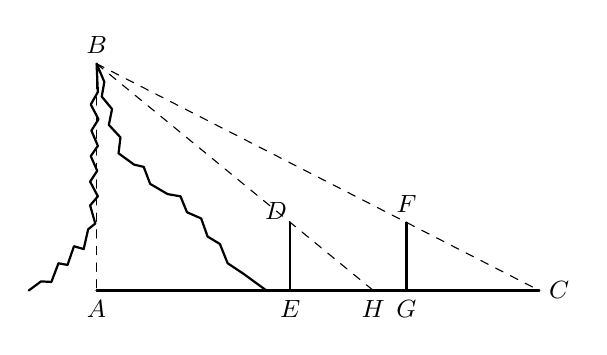
\begin{tikzpicture}[x=0.82cm,y=0.72cm,line cap=round,line join=round,font=\small]
  \coordinate (A) at (0,0);
  \coordinate (B) at (0,4);
  \coordinate (E) at (3,0);
  \coordinate (D) at (3,1.2);
  \coordinate (H) at (4.286,0);
  \coordinate (G) at (4.8,0);
  \coordinate (F) at (4.8,1.2);
  \coordinate (C) at (6.857,0);

  % Island outline and measured height
  \draw[thick]
    (-1.05,0) -- (-0.86,0.16) -- (-0.70,0.15) -- (-0.59,0.48)
    -- (-0.45,0.45) -- (-0.35,0.78) -- (-0.20,0.73) -- (-0.13,1.08)
    -- (-0.02,1.18) -- (-0.10,1.50) -- (0.02,1.66) -- (-0.10,1.92)
    -- (0.01,2.11) -- (-0.09,2.37) -- (0.02,2.55) -- (-0.08,2.82)
    -- (0.03,3.02) -- (-0.09,3.28) -- (0.02,3.50) -- (0,4)
    -- (0.12,3.68) -- (0.08,3.42) -- (0.24,3.20) -- (0.19,2.92)
    -- (0.37,2.70) -- (0.34,2.42) -- (0.58,2.22) -- (0.73,2.18)
    -- (0.83,1.88) -- (1.10,1.70) -- (1.30,1.66) -- (1.40,1.38)
    -- (1.62,1.27) -- (1.72,0.95) -- (1.91,0.82) -- (2.03,0.48)
    -- (2.28,0.29) -- (2.63,0);
  \draw[dashed] (B) -- (A);

  % Horizontal reference line, equal poles and sight lines
  \draw[thick] (A) -- (C);
  \draw[dashed] (B) -- (H);
  \draw[dashed] (B) -- (C);
  \draw[thick] (D) -- (E);
  \draw[thick] (F) -- (G);

  \node[above] at (B) {$B$};
  \node[below] at (A) {$A$};
  \node[above left,inner sep=1pt] at (D) {$D$};
  \node[below] at (E) {$E$};
  \node[below] at (H) {$H$};
  \node[above] at (F) {$F$};
  \node[below] at (G) {$G$};
  \node[right] at (C) {$C$};
\end{tikzpicture}
\end{center}
\nopagebreak[4]
\begin{gkopts}(1)
\task A．$\dfrac{\text{\text{表高}}\times\text{\text{表距}}}{\text{\text{表目距的差}}}+\text{\text{表高}}$
\task B．$\dfrac{\text{\text{表高}}\times\text{\text{表距}}}{\text{\text{表目距的差}}}-\text{\text{表高}}$
\task C．$\dfrac{\text{\text{表高}}\times\text{\text{表距}}}{\text{\text{表目距的差}}}+\text{\text{表距}}$
\task D．$\dfrac{\text{\text{表高}}\times\text{\text{表距}}}{\text{\text{表目距的差}}}-\text{\text{表距}}$
\end{gkopts}

\Needspace{4\baselineskip}
\textbf{解析}

记表高为 $h$、表距 $d=EG$。由图，$A,E,H,G,C$ 依次在同一水平线上，$B,D,H$ 共线，$B,F,C$ 共线，且 $DE=FG=h$。

相似三角形给出
$\dfrac{AB}{AH}=\dfrac{h}{EH}$、
$\dfrac{AB}{AC}=\dfrac{h}{GC}$。
又 $AH=AE+EH$、$AC=AG+GC$，故
$AB=h+h\dfrac{AE}{EH}=h+h\dfrac{AG}{GC}$，
并有 $\dfrac{AE}{EH}=\dfrac{AG}{GC}$。消去 $AE,AG$ 后得到
$\dfrac{EG}{GC-EH}=\dfrac{AG}{GC}$，于是
$AB=h+\dfrac{h\cdot EG}{GC-EH}$，对应选项 A。

\gkanswer{答案：A}

\end{answer}
\begin{answer}
\gksolhead{10}{}

\textbf{题目}：

设 $a\ne0$，若 $x=a$ 是函数 $f(x)=a(x-a)^2(x-b)$ 的极大值点，则\mbox{（　　）}

\begin{gkopts}(4)
\task A．$a<b$
\task B．$a>b$
\task C．$ab<a^2$
\task D．$ab>a^2$
\end{gkopts}

\Needspace{4\baselineskip}
\textbf{解析}

在 $x=a$ 附近令 $u=x-a$，则
$f(x)=a u^2(a-b+u)=a(a-b)u^2+a u^3$。
要使 $u=0$ 为局部极大值点，首个非零偶次项系数须为负，即 $a(a-b)<0$。因 $a\ne0$，这等价于 $a^2<ab$，选 D。

\gkanswer{答案：D}

\end{answer}
\begin{answer}
\gksolhead{11}{}

\textbf{题目}：

设 $B$ 是椭圆 $C:\dfrac{x^2}{a^2}+\dfrac{y^2}{b^2}=1\ (a>b>0)$ 的上顶点，若 $C$ 上任意一点 $P$ 都满足 $|PB|\leqslant2b$，则 $C$ 的离心率的取值范围是\mbox{（　　）}

\begin{gkopts}(2)
\task A．$\left[\dfrac{\sqrt2}{2},1\right)$
\task B．$\left[\dfrac12,1\right)$
\task C．$\left(0,\dfrac{\sqrt2}{2}\right]$
\task D．$\left(0,\dfrac12\right]$
\end{gkopts}

\Needspace{4\baselineskip}
\textbf{解析}

设 $c^2=a^2-b^2$，并令 $t=\sin\theta$。椭圆点 $P=(a\cos\theta,b\sin\theta)$ 到上顶点 $B=(0,b)$ 的距离满足
$|PB|^2=a^2+b^2-c^2t^2-2b^2t$，其中 $-1\leqslant t\leqslant1$。

这是关于 $t$ 的开口向下二次函数，顶点在 $t_0=-b^2/c^2$。若 $c^2\leqslant b^2$，顶点不在区间内部，区间最大值在 $t=-1$ 处取 $4b^2$，满足条件；若 $c^2>b^2$，顶点在区间内部，最大值为 $a^2+b^2+b^4/c^2$，严格大于 $4b^2$，不满足条件。

所以条件等价于 $c^2\leqslant b^2$，即 $e^2=c^2/a^2\leqslant1/2$。结合椭圆 $e>0$，取值范围为 $(0,\sqrt2/2]$，选 C。

\gkanswer{答案：C}

\end{answer}
\begin{answer}
\gksolhead{12}{}

\textbf{题目}：

设 $a=2\ln1.01$，$b=\ln1.02$，$c=\sqrt{1.04}-1$，则\mbox{（　　）}

\begin{gkopts}(4)
\task A．$a<b<c$
\task B．$b<c<a$
\task C．$b<a<c$
\task D．$c<a<b$
\end{gkopts}

\Needspace{4\baselineskip}
\textbf{解析}

$a=2\ln1.01=\ln(1.01)^2=\ln1.0201>\ln1.02=b$。另外
$b\approx0.01980263$，$c=\sqrt{1.04}-1\approx0.01980390$，所以 $b<c<a$，选 B。

\gkanswer{答案：B}

\par\medskip

\end{answer}
\gkpart{二、填空题}

\begin{answer}
\gksolhead{13}{}

\textbf{题目}：

已知双曲线 $C:\dfrac{x^2}{m}-y^2=1\ (m>0)$ 的一条渐近线为 $\sqrt3x+my=0$，则 $C$ 的焦距为 $\underline{\qquad\qquad}$．

\Needspace{4\baselineskip}
\textbf{解析}

双曲线 $x^2/m-y^2=1$ 的渐近线斜率为 $\pm1/\sqrt m$。给定直线 $\sqrt3x+my=0$ 的斜率为 $-\sqrt3/m$，从而
$\sqrt3/m=1/\sqrt m$，得 $m=3$。
双曲线的焦半距 $c=\sqrt{m+1}=2$，故焦距 $2c=4$。

\gkanswer{答案：$4$}

\end{answer}
\begin{answer}
\gksolhead{14}{}

\textbf{题目}：

已知向量 $\boldsymbol a=(1,3)$，$\boldsymbol b=(3,4)$，$(\boldsymbol a-\lambda\boldsymbol b)\perp\boldsymbol b$，则 $\lambda=$ $\underline{\qquad\qquad}$．

\Needspace{4\baselineskip}
\textbf{解析}

由 $(\boldsymbol a-\lambda\boldsymbol b)\cdot\boldsymbol b=0$，
$\lambda=(\boldsymbol a\cdot\boldsymbol b)/(\boldsymbol b\cdot\boldsymbol b)$。
计算 $\boldsymbol a\cdot\boldsymbol b=1\cdot3+3\cdot4=15$、$\boldsymbol b\cdot\boldsymbol b=3^2+4^2=25$，故 $\lambda=3/5$。

\gkanswer{答案：$\dfrac35$}

\end{answer}
\begin{answer}
\gksolhead{15}{}

\textbf{题目}：

记 $\triangle ABC$ 的内角 $A,B,C$ 的对边分别为 $a,b,c$，面积为 $\sqrt3$，$B=60^\circ$，$a^2+c^2=3ac$，则 $b=$ $\underline{\qquad\qquad}$．

\Needspace{4\baselineskip}
\textbf{解析}

面积公式给出 $\sqrt3=\frac12ac\sin60^\circ=\frac{\sqrt3}{4}ac$，所以 $ac=4$。余弦定理得
$b^2=a^2+c^2-2ac\cos60^\circ=3ac-ac=2ac=8$，
故 $b=2\sqrt2$。

\gkanswer{答案：$2\sqrt2$}

\end{answer}
\begin{answer}
\gksolhead{16}{}

\textbf{题目}：

以图①为正视图，在图②③④⑤中选两个分别作为侧视图和俯视图，组成某个三棱锥的三视图，则所选侧视图和俯视图的编号依次为 $\underline{\qquad\qquad}$．（写出符合要求的一组答案即可）
\nopagebreak[4]
\begin{center}% 2021 全国乙卷理科第 16 题：正视图与候选侧视图、俯视图；逻辑图名 2021-national-b-science-t16-views
\begin{tikzpicture}[x=0.72cm,y=0.72cm,line cap=round,line join=round,font=\small]
  % Front view (figure 1)
  \coordinate (a1) at (0,0);
  \coordinate (b1) at (2,0);
  \coordinate (c1) at (2,1);
  \draw[thick] (a1) -- (b1) -- (c1) -- cycle;
  \draw (0,-0.08) -- (0,-0.30);
  \draw (2,-0.08) -- (2,-0.30);
  \draw[<->] (0,-0.25) -- (2,-0.25) node[midway,below,inner sep=1pt] {$2$};
  \draw (2.08,0) -- (2.34,0);
  \draw (2.08,1) -- (2.34,1);
  \draw[<->] (2.27,0) -- (2.27,1) node[midway,right,inner sep=1pt] {$1$};
  \node[below] at (1,-0.62) {图①};

  % Side-view option 2: visible central edge
  \coordinate (a2) at (3.45,0);
  \coordinate (b2) at (5.45,0);
  \coordinate (c2) at (4.45,1);
  \draw[thick] (a2) -- (b2) -- (c2) -- cycle;
  \draw[thick] (c2) -- (4.45,0);
  \draw (3.45,-0.08) -- (3.45,-0.30);
  \draw (5.45,-0.08) -- (5.45,-0.30);
  \draw[<->] (3.45,-0.25) -- (5.45,-0.25) node[midway,below,inner sep=1pt] {$2$};
  \draw (5.53,0) -- (5.78,0);
  \draw (5.53,1) -- (5.78,1);
  \draw[<->] (5.72,0) -- (5.72,1) node[midway,right,inner sep=1pt] {$1$};
  \node[below] at (4.45,-0.62) {图②};

  % Side-view option 3: hidden central edge
  \coordinate (a3) at (7.05,0);
  \coordinate (b3) at (9.05,0);
  \coordinate (c3) at (8.05,1);
  \draw[thick] (a3) -- (b3) -- (c3) -- cycle;
  \draw[dashed] (c3) -- (8.05,0);
  \draw (7.05,-0.08) -- (7.05,-0.30);
  \draw (9.05,-0.08) -- (9.05,-0.30);
  \draw[<->] (7.05,-0.25) -- (9.05,-0.25) node[midway,below,inner sep=1pt] {$2$};
  \draw (9.13,0) -- (9.38,0);
  \draw (9.13,1) -- (9.38,1);
  \draw[<->] (9.32,0) -- (9.32,1) node[midway,right,inner sep=1pt] {$1$};
  \node[below] at (8.05,-0.62) {图③};

  % Top-view options are shifted down to keep their geometry clear of the upper-row labels.
  \begin{scope}[yshift=-0.5cm]
  % Top-view option 4
  \coordinate (a4) at (0,-2.65);
  \coordinate (b4) at (0,-0.65);
  \coordinate (c4) at (2,-1.65);
  \draw[thick] (a4) -- (b4) -- (c4) -- cycle;
  \draw (-0.08,-2.65) -- (-0.34,-2.65);
  \draw (-0.08,-0.65) -- (-0.34,-0.65);
  \draw[<->] (-0.27,-2.65) -- (-0.27,-0.65) node[midway,left,inner sep=1pt] {$2$};
  \draw (0,-2.73) -- (0,-2.96);
  \draw (2,-1.73) -- (2,-2.96);
  \draw[<->] (0,-2.88) -- (2,-2.88) node[midway,below,inner sep=1pt] {$2$};
  \node[below] at (1,-3.22) {图④};

  % Top-view option 5, with the visible median
  \coordinate (a5) at (5.25,-0.65);
  \coordinate (b5) at (5.25,-2.65);
  \coordinate (c5) at (3.25,-1.65);
  \draw[thick] (a5) -- (b5) -- (c5) -- cycle;
  \draw[thick] (c5) -- (5.25,-1.65);
  \draw (5.33,-2.65) -- (5.58,-2.65);
  \draw (5.33,-0.65) -- (5.58,-0.65);
  \draw[<->] (5.50,-2.65) -- (5.50,-0.65) node[midway,right,inner sep=1pt] {$2$};
  \draw (3.25,-1.73) -- (3.25,-2.96);
  \draw (5.25,-2.73) -- (5.25,-2.96);
  \draw[<->] (3.25,-2.88) -- (5.25,-2.88) node[midway,below,inner sep=1pt] {$2$};
  \node[below] at (4.25,-3.22) {图⑤};
  \end{scope}
\end{tikzpicture}
\end{center}
\nopagebreak[4]
\Needspace{4\baselineskip}
\textbf{解析}

取底面三个顶点坐标为 $A=(0,0,0)$、$B=(0,2,0)$、$C=(2,1,0)$，顶点 $P=(2,1,1)$。沿 $y$ 方向作正视投影时，$A,B$ 重合于 $(0,0)$，$C,P$ 投影为 $(2,0),(2,1)$，得到图①。

从 $x=2$ 一侧向 $x=0$ 看，底边投影从 $y=0$ 到 $y=2$，顶点与 $C$ 的投影重合在 $y=1$，且棱 $CP$ 可见，得到带实线中线的图②；从 $x=0$ 一侧向 $x=2$ 看，$CP$ 被遮挡，得到虚线中线的图③。俯视时 $P$ 投影与 $C$ 重合，外轮廓为图④。因此题目所需的一组可取②、④；若按左侧观察则取③、④。

\gkanswer{答案：侧视图②，俯视图④}

\par\medskip

\end{answer}
\gkpart{三、解答题}

\begin{answer}
\gksolhead{17}{}

\textbf{题目}：

某厂研制了一种生产高精产品的设备，为检验新设备生产产品的某项指标有无提高，用一台旧设备和一台新设备各生产了 $10$ 件产品，得到各件产品该项指标数据如下：

\begin{center}
\begingroup\setlength{\tabcolsep}{4pt}
\begin{tabular}{crrrrrrrrrr}
\toprule
设备 & 1 & 2 & 3 & 4 & 5 & 6 & 7 & 8 & 9 & 10 \\
\midrule
旧设备 & $9.8$ & $10.3$ & $10.0$ & $10.2$ & $9.9$ & $9.8$ & $10.0$ & $10.1$ & $10.2$ & $9.7$ \\
新设备 & $10.1$ & $10.4$ & $10.1$ & $10.0$ & $10.1$ & $10.3$ & $10.6$ & $10.5$ & $10.4$ & $10.5$ \\
\bottomrule
\end{tabular}
\endgroup
\end{center}

旧设备和新设备生产产品的该项指标的样本平均值分别记为 $\bar x$ 和 $\bar y$，样本方差分别记为 $s_1^2$ 和 $s_2^2$。

  (1) 求 $\bar x,\bar y,s_1^2,s_2^2$；

  (2) 判断新设备生产产品的该项指标的均值较旧设备是否有显著提高（如果 $\bar y-\bar x\geqslant2\sqrt{\dfrac{s_1^2+s_2^2}{10}}$，则认为新设备生产产品的该项指标的均值较旧设备有显著提高，否则不认为有显著提高）．

\Needspace{4\baselineskip}
\textbf{解析}

\textbf{(1) 样本平均值与方差}

\Needspace{5\baselineskip}
旧设备数据和为 $100$，故 $\bar x=10$。相对均值的偏差为
\nopagebreak[4]
\[
\begin{aligned}
&(-0.2,0.3,0,0.2,-0.1,\\
&\quad -0.2,0,0.1,0.2,-0.3).
\end{aligned}
\]
平方和为 $0.36$，所以按样本方差定义 $s_1^2=0.36/10=0.036$。

\Needspace{5\baselineskip}
新设备数据和为 $103$，故 $\bar y=10.3$。相对均值的偏差为
\nopagebreak[4]
\[
\begin{aligned}
&(-0.2,0.1,-0.2,-0.3,-0.2,\\
&\quad 0,0.3,0.2,0.1,0.2).
\end{aligned}
\]
平方和为 $0.40$，所以 $s_2^2=0.40/10=0.040$。

\textbf{(2) 均值是否显著提高}

$\bar y-\bar x=0.3$，阈值为
$2\sqrt{\dfrac{0.036+0.040}{10}}=2\sqrt{0.0076}\approx0.1744$。
因 $0.3\geqslant0.1744$，依题设判据认为新设备生产产品该指标的均值较旧设备有显著提高。

\gkanswer{答案（1）：$\bar x=10,\ \bar y=10.3,\ s_1^2=0.036,\ s_2^2=0.040$}

\gkanswer{答案（2）：新设备指标均值有显著提高}

\end{answer}
\begin{answer}
\gksolhead{18}{}

\textbf{题目}：

如图，四棱锥 $P-ABCD$ 的底面是矩形，$PD\perp$ 底面 $ABCD$，$PD=DC=1$，$M$ 为 $BC$ 的中点，且 $PB\perp AM$。
\nopagebreak[4]
\begin{center}% 2021 全国乙卷理科第 18 题：四棱锥 P-ABCD，底面 ABCD 为矩形；逻辑图名 2021-national-b-science-t18-pyramid
% 隐藏棱 AD、DC、PD 以虚线表示；M 为 BC 中点，连结 PM。
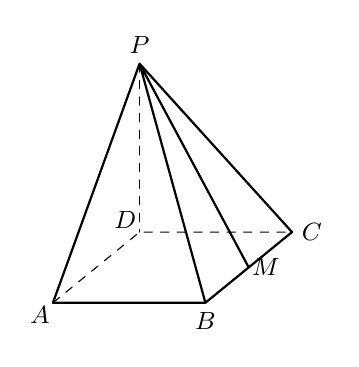
\begin{tikzpicture}[x=0.88cm,y=0.88cm,line cap=round,line join=round,font=\small]
  \coordinate (A) at (0,0);
  \coordinate (B) at (2.2,0);
  \coordinate (C) at (3.45,1.02);
  \coordinate (D) at (1.25,1.02);
  \coordinate (P) at (1.25,3.45);
  \coordinate (M) at (2.825,0.51);

  % Visible base and lateral edges
  \draw[thick] (A) -- (B) -- (C);
  \draw[thick] (P) -- (A) (P) -- (B) (P) -- (C) (P) -- (M);

  % Hidden rear edges
  \draw[dashed] (A) -- (D) -- (C);
  \draw[dashed] (P) -- (D);

  \node[above] at (P) {$P$};
  \node[below left,inner sep=1pt] at (A) {$A$};
  \node[below] at (B) {$B$};
  \node[right] at (C) {$C$};
  \node[above left,inner sep=1pt] at (D) {$D$};
  \node[right,inner sep=1pt] at (M) {$M$};
\end{tikzpicture}
\end{center}
\nopagebreak[4]
  (1) 求 $BC$；

  (2) 求二面角 $A-PM-B$ 的正弦值。

\Needspace{4\baselineskip}
\textbf{解析}

以矩形底面建立直角坐标系：令 $A=(0,0,0)$、$B=(1,0,0)$、$C=(1,d,0)$、$D=(0,d,0)$。因 $DC=1$，矩形对边相等，故 $AB=1$；又 $PD\perp ABCD$、$PD=1$，所以 $P=(0,d,1)$。$M$ 为 $BC$ 中点，故 $M=(1,d/2,0)$。

\textbf{(1)} $\overrightarrow{PB}=(1,-d,-1)$，$\overrightarrow{AM}=(1,d/2,0)$。由垂直条件
$\overrightarrow{PB}\cdot\overrightarrow{AM}=1-d^2/2=0$，
得 $d=\sqrt2$，所以 $BC=\sqrt2$。

\textbf{(2)} 代入 $d=\sqrt2$，从 $M$ 出发取
$\overrightarrow{MP}=(-1,1/\sqrt2,1)$、
$\overrightarrow{MA}=(-1,-1/\sqrt2,0)$、
$\overrightarrow{MB}=(0,-1/\sqrt2,0)$。
平面 $APM$ 与 $BPM$ 的法向量可分别取
$\boldsymbol n_1=\overrightarrow{MP}\times\overrightarrow{MA}=(1/\sqrt2,-1,\sqrt2)$，
$\boldsymbol n_2=\overrightarrow{MP}\times\overrightarrow{MB}=(1/\sqrt2,0,1/\sqrt2)$。

$|\boldsymbol n_1|=\sqrt{7/2}$、$|\boldsymbol n_2|=1$，且 $\boldsymbol n_1\cdot\boldsymbol n_2=3/2$。两个平面的夹角与所求二面角可能互为补角，但正弦相同，故
$\sin\angle(A-PM-B)=\sqrt{1-\left(\dfrac{3}{\sqrt{14}}\right)^2}=\sqrt{\dfrac5{14}}$。

\gkanswer{答案（1）：$BC=\sqrt2$}

\gkanswer{答案（2）：$\sin\angle(A-PM-B)=\sqrt{\dfrac5{14}}$}

\end{answer}
\begin{answer}
\gksolhead{19}{}

\textbf{题目}：

记 $S_n$ 为数列 $\{a_n\}$ 的前 $n$ 项和，$b_n$ 为数列 $\{S_n\}$ 的前 $n$ 项积，已知 $\dfrac2{S_n}+\dfrac1{b_n}=2$。

  (1) 证明：数列 $\{b_n\}$ 是等差数列；

  (2) 求 $\{a_n\}$ 的通项公式。

\Needspace{4\baselineskip}
\textbf{解析}

\textbf{(1)} 由 $b_1=S_1$，原条件在 $n=1$ 时给出 $2/S_1+1/S_1=2$，所以 $S_1=b_1=3/2$。

当 $n\geqslant2$ 时，$b_n=b_{n-1}S_n$。将原式乘以 $S_n$：
$2+S_n/b_n=2S_n$，而 $S_n/b_n=1/b_{n-1}$，于是
$S_n=1+1/(2b_{n-1})$。因此
$b_n=b_{n-1}S_n=b_{n-1}+1/2$。

\textbf{(2)} 故 $\{b_n\}$ 是首项 $3/2$、公差 $1/2$ 的等差数列，$b_n=(n+2)/2$。由 $S_n=b_n/b_{n-1}$ 得 $S_n=(n+2)/(n+1)$（$n\geqslant2$，$n=1$ 也符合）。于是
$a_1=S_1=3/2$，且对 $n\geqslant2$，
$a_n=S_n-S_{n-1}=\dfrac{n+2}{n+1}-\dfrac{n+1}{n}=-\dfrac1{n(n+1)}$。

\gkanswer{答案（1）：$\{b_n\}$ 是首项 $\dfrac32$、公差 $\dfrac12$ 的等差数列，$b_n=\dfrac{n+2}{2}$}

\gkanswer{答案（2）：$a_1=\dfrac32,\ a_n=-\dfrac1{n(n+1)}\ (n\geqslant2)$}

\end{answer}
\begin{answer}
\gksolhead{20}{}

\textbf{题目}：

设函数 $f(x)=\ln(a-x)$，已知 $x=0$ 是函数 $y=xf(x)$ 的极值点。

  (1) 求 $a$；

  (2) 设函数 $g(x)=\dfrac{x+f(x)}{xf(x)}$，证明：$g(x)<1$。

\Needspace{4\baselineskip}
\textbf{解析}

\textbf{(1)} 令 $h(x)=x\ln(a-x)$，定义域为 $x<a$。在 $x=0$ 可导，且
$h'(0)=\ln a$。极值点是驻点，故 $\ln a=0$，得到 $a=1$。

\textbf{(2)} 此时 $f(x)=\ln(1-x)$，$x<1$。$g$ 的定义域还须排除 $x=0$。令 $t=1-x$，则 $t>0,t\ne1$。设 $\phi(t)=t\ln t-t+1$，代入并整理得
$g(x)-1=\dfrac{1-t+t\ln t}{x\ln t}=\dfrac{\phi(t)}{x\ln t}$。
函数 $\phi(t)$ 在 $t>0$ 上以 $t=1$ 为唯一最小点，最小值为 $0$，所以 $\phi(t)>0$（$t\ne1$）。当 $x<0$ 时 $t>1$，分母 $x\ln t<0$；当 $0<x<1$ 时 $0<t<1$，分母同样为负。因此 $g(x)-1<0$，即 $g(x)<1$。

\gkanswer{答案（1）：$a=1$}

\gkanswer{答案（2）：在定义域内 $g(x)<1$}

\end{answer}
\begin{answer}
\gksolhead{21}{}

\textbf{题目}：

已知抛物线 $C:x^2=2py\ (p>0)$ 的焦点为 $F$，且 $F$ 与圆 $M:x^2+(y+4)^2=1$ 上的点的距离的最小值为 $4$。

  (1) 求 $p$；

  (2) 若点 $P$ 在圆 $M$ 上，$PA,PB$ 是 $C$ 的两条切线，$A,B$ 是切点，求 $\triangle PAB$ 面积的最大值。

\Needspace{4\baselineskip}
\textbf{解析}

\textbf{(1)} 抛物线 $x^2=2py$ 的焦点为 $F=(0,p/2)$。圆心 $M=(0,-4)$、半径为 $1$。因 $p>0$，焦点到圆上点的最小距离为 $FM-1=p/2+4-1$。令其等于 $4$，得 $p=2$。

\textbf{(2)} 当 $p=2$ 时，抛物线为 $x^2=4y$。用参数 $t$ 表示切点 $A=(2t,t^2)$，其切线为 $y=tx-t^2$。设 $P=(u,v)$，从 $P$ 引出的两条切线参数 $t_1,t_2$ 满足
$t^2-ut+v=0$，故 $t_1+t_2=u$、$t_1t_2=v$。

\Needspace{5\baselineskip}
由行列式，三角形面积为
\nopagebreak[4]
\[
\begin{aligned}
[\triangle PAB]&=\dfrac12\left|\det(A-P,B-P)\right|\\
&=\dfrac12(u^2-4v)^{3/2}.
\end{aligned}
\]
这里 $v<0$，且根差的绝对值为 $\sqrt{u^2-4v}$。

点 $P$ 在圆上，$u^2+(v+4)^2=1$。令 $r=v+4\in[-1,1]$，则
$u^2-4v=1-r^2-4(r-4)=17-4r-r^2$。
该式在 $[-1,1]$ 上递减，最大值在 $r=-1$ 取 $20$。因此
$[\triangle PAB]_{\max}=\dfrac12\cdot20^{3/2}=20\sqrt5$。

\gkanswer{答案（1）：$p=2$}

\gkanswer{答案（2）：$[\triangle PAB]_{\max}=20\sqrt5$}

\end{answer}
\begin{answer}
\gksolhead{22}{}

\textbf{题目}：

在直角坐标系 $xOy$ 中，$\odot C$ 的圆心为 $C(2,1)$，半径为 $1$。

  (1) 写出 $\odot C$ 的一个参数方程；

  (2) 过点 $F(4,1)$ 作 $\odot C$ 的两条切线，以坐标原点为极点，$x$ 轴正半轴为极轴建立极坐标系，求这两条切线的极坐标方程。

\Needspace{4\baselineskip}
\textbf{解析}

\textbf{(1)} 圆心 $(2,1)$、半径 $1$，可取参数方程
$\begin{cases}x=2+\cos t,\\y=1+\sin t,\end{cases}\quad 0\leqslant t<2\pi$。

\textbf{(2)} 设切点的半径方向单位向量为 $(\cos\theta,\sin\theta)$。对应切线为
$\cos\theta(x-2)+\sin\theta(y-1)=1$。
切线过 $F(4,1)$，故 $2\cos\theta=1$，于是 $\cos\theta=1/2$、$\sin\theta=\pm\sqrt3/2$。得到两条直线
$x+\sqrt3y=4+\sqrt3$ 和 $x-\sqrt3y=4-\sqrt3$。

代入 $x=\rho\cos\theta,\ y=\rho\sin\theta$，所求极坐标方程为
$\rho(\cos\theta+\sqrt3\sin\theta)=4+\sqrt3$，
$\rho(\cos\theta-\sqrt3\sin\theta)=4-\sqrt3$。

\gkanswer{答案（1）：$\begin{cases}x=2+\cos t,\\y=1+\sin t,\end{cases}\quad 0\leqslant t<2\pi$}

\gkanswer{答案（2）：$\rho(\cos\theta+\sqrt3\sin\theta)=4+\sqrt3$、$\rho(\cos\theta-\sqrt3\sin\theta)=4-\sqrt3$}

\end{answer}
\begin{answer}
\gksolhead{23}{}

\textbf{题目}：

已知函数 $f(x)=|x-a|+|x+3|$。

  (1) 当 $a=1$ 时，求不等式 $f(x)\geqslant6$ 的解集；

  (2) 若 $f(x)>-a$，求 $a$ 的取值范围。

\makeatletter\def\gkanswerblock{answer}\ifx\@currenvir\gkanswerblock\else\clearpage\fi\makeatother

\Needspace{4\baselineskip}
\textbf{解析}

\textbf{(1)} 当 $a=1$ 时，
$f(x)=|x-1|+|x+3|$。在 $-3\leqslant x\leqslant1$ 时，两距离之和为 $4$；在 $x<-3$ 时 $f(x)=-2x-2$；在 $x>1$ 时 $f(x)=2x+2$。所以 $f(x)\geqslant6$ 等价于 $x\leqslant-4$ 或 $x\geqslant2$，解集为
$(-\infty,-4]\cup[2,+\infty)$。

原卷第 1142 页此题未附函数图。下图仅为解析辅助，不属于试题或简答版题面。
\nopagebreak[4]
\begin{center}% 2021 全国乙卷理科第 23 题的作图网格（补充解题辅助图）。
% 原卷 PDF 第 2 页未附坐标网格；本图按 a=1 绘出 f(x)=|x-1|+|x+3| 与 y=6。
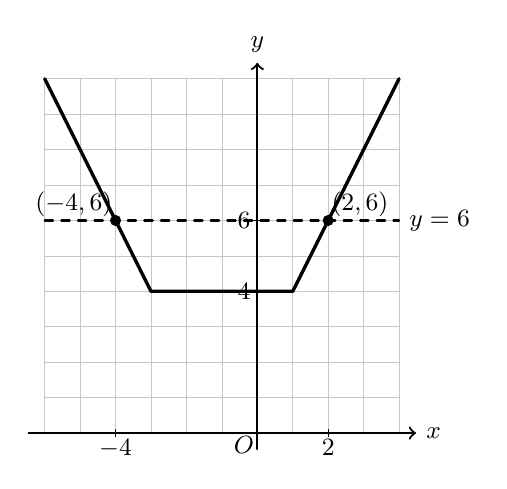
\begin{tikzpicture}[x=0.45cm,y=0.45cm,line cap=round,line join=round,font=\small]
  % Unit grid
  \draw[gray!45,line width=0.25pt] (-6,0) grid[step=1] (4,10);

  % Axes
  \draw[->,thick] (-6.45,0) -- (4.48,0) node[right] {$x$};
  \draw[->,thick] (0,-0.45) -- (0,10.45) node[above] {$y$};
  \node[below left,inner sep=1pt] at (0,0) {$O$};

  % Unit marks and the two boundary abscissas
  \foreach \x in {-4,2} {
    \draw (\x,0.10) -- (\x,-0.10);
    \node[below,inner sep=1pt] at (\x,-0.10) {$\x$};
  }
  \foreach \y in {4,6} {
    \draw (0.10,\y) -- (-0.10,\y);
    \node[left,inner sep=1pt] at (-0.10,\y) {$\y$};
  }

  % f(x)=|x-1|+|x+3| and the comparison level y=6
  \draw[dashed,thick] (-6,6) -- (4,6) node[right] {$y=6$};
  \draw[very thick] (-6,10) -- (-3,4) -- (1,4) -- (4,10);
  \fill (-4,6) circle (2pt);
  \fill (2,6) circle (2pt);
  \node[above right,inner sep=1pt] at (2,6) {$(2,6)$};
  \node[above left,inner sep=1pt] at (-4,6) {$(-4,6)$};
\end{tikzpicture}
\end{center}
\nopagebreak[4]
\textbf{(2) 说明：}原题只写“若 $f(x)>-a$”，没有标明 $x$ 的量词，因此存在两种不同结论。

若理解为对任意实数 $x$ 恒成立，则 $f(x)=|x-a|+|x+3|$ 的最小值 $|a+3|$ 必须大于 $-a$，即 $|a+3|>-a$。当 $a<-3$ 时不成立；当 $a\geqslant-3$ 时化为 $a+3>-a$，得 $a>-3/2$。

若理解为存在实数 $x$ 使 $f(x)>-a$，由于 $f(x)\to+\infty$（$|x|\to+\infty$），任意实数 $a$ 都存在满足条件的 $x$，取值范围为 $\mathbf R$。没有权威同版材料澄清前，不能从原句唯一确定范围。

\gkanswer{答案（1）：$(-\infty,-4]\cup[2,+\infty)$}

\gkanswer{答案（2）：见解析版}

\end{answer}